\section{Določanje števila $\mathbf{\pi}$}

Splošno znan je Monte-Carlovski način aproksimacije števila $\pi$. Razmerje med številom točk v enotskem krogu in v kvadratu, kateremu je včrtan krog je natanko $\frac{\pi}{4}$. Tako smo naredili ta preprosti algoritem in aproksimirali $\pi$, pri čemer smo uporabili naključno generirano in ``regularno'' mrežo točk ter poenostavitev zaradi simetrije.

Pri tem smo napako metode računali računali po poenostavljenem splošnem pravilu:
\begin{equation}
    \pi \approx \hat{\theta} \pm \sigma = 4 \, \frac{n}{N} \pm \frac{\hat{\theta}}{\sqrt{N}} \sqrt{n-\frac{n^2}{N}}
\end{equation}
kjer je $\hat{\theta}$ izračunana vrednost, $n$ število zadetkov znotraj kroga in $N$ število vseh zadetkov znotraj kvadrata. Tako dobimo rezultate vidne na spodnji sliki, kjer MMC zaradi naključnosti ``pleše'' okoli prave vrednosti, v primeru regularne mreže pa lepo konvergira, kar bi se dalo analitično popisati v odvisnosti od diskretizacije. Potrebno je tudi poudariti, da je tak iračun pribl. še enkrat hitrejši od naključnega.

\begin{figure}[ht]
    \centering
    \begin{minipage}{0.35\textwidth}
        \centering
        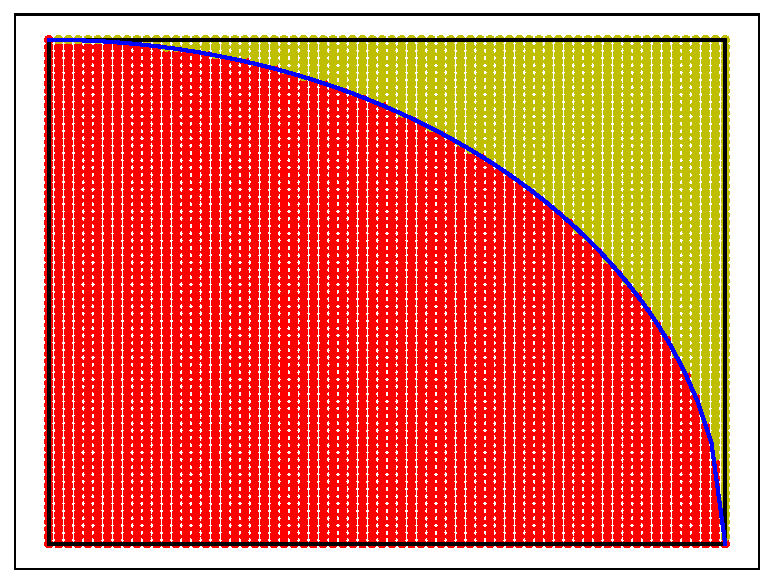
\includegraphics[width=0.9\linewidth]{7. nal slike/pi_mreža.pdf}
        \caption[short]{``regularna'' mreža}
    \end{minipage}
    \begin{minipage}{0.35\textwidth}
        \centering
        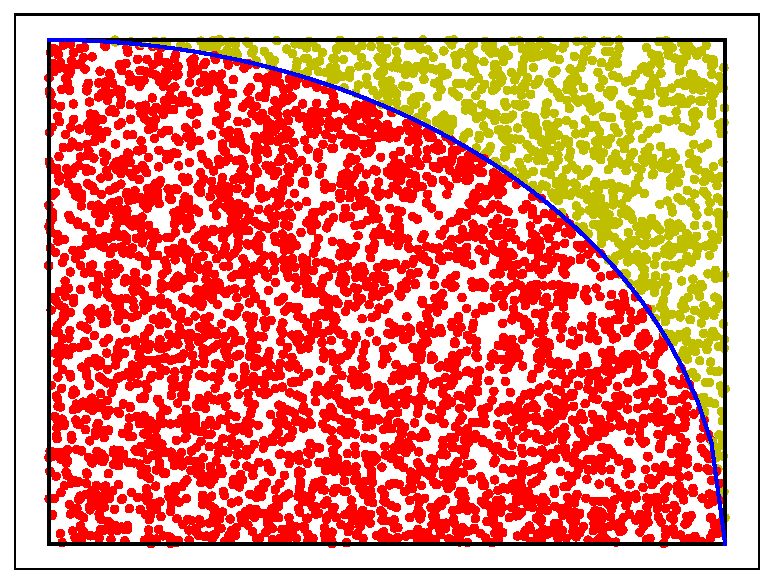
\includegraphics[width=0.9\linewidth]{7. nal slike/pi.pdf}
        \caption[short]{naključna mreža}
    \end{minipage}
\end{figure}
\begin{figure}[ht]
    \centering
    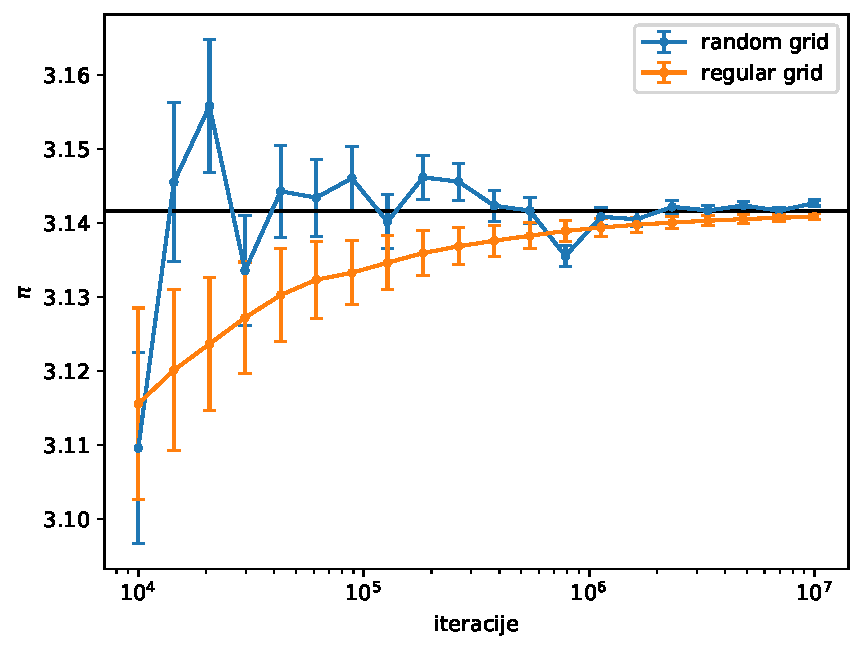
\includegraphics[width=0.45\textwidth]{7. nal slike/pi_napaka.pdf}
    \caption[short]{Napaka in rezultat simulacije v odvisnosti od števila iteracij.}
\end{figure}

\section{Določanje mase telesa}
\setcounter{figure}{0}

Ako je telo podano le s ploskvami, ki ga omejujejo, je mogoče njegovo prostornino z integracijo izračunati:
\begin{equation}
    V=\int_V f(x,y,z) \,dV
\end{equation}
kjer je $f(x,y,z)$ zvezna funkcija, ki opisuje omejujočo ploskev. Ako je $f$ nezvezna jo lahko razdelimo na odsekoma zvezne dele. Ker so večkratni integrali lahko zahtevni imamo mnogo numeričnih metod, s katerimi si lahko pomagamo. Ena izmed njih je metoda Monte Carlo (MMC).

Maso takega poljubnega telesa lahko določimo kot 
\begin{equation}
    m=\rho\,V
\end{equation}
v homogenem primeru, ko je gostota konstantna po celi prostornini. Ako ni konstantna, vržemo funkcijsko odvisnost $\rho(x,y,z)$ v integral za prostornino, ki ga računamo z MMC:
\begin{equation}
    m=\int_V \rho(x,y,z)\,f(x,y,z) \,dV
\end{equation}

Dano je telo, ki ga omejuje ploskev $\sqrt{|x|}+\sqrt{|y|}+\sqrt{|z|}=1$, bomo obravnavali na kvadratnem območju od -1 do +1 v vsaki osi. Sicer bi bilo mogoče, kot je že iz oblike enačbe in spodnje slike razvidno, z obravnavo v sferi zmanjšati število neuspešnih izračunov, bi to pomenilo, da moramo prilagoditi nakjučno porazdelitev in enačbo v sferično obliko, za kar pa nam zmanjkuje časa...

\begin{figure}[ht]
    \centering
    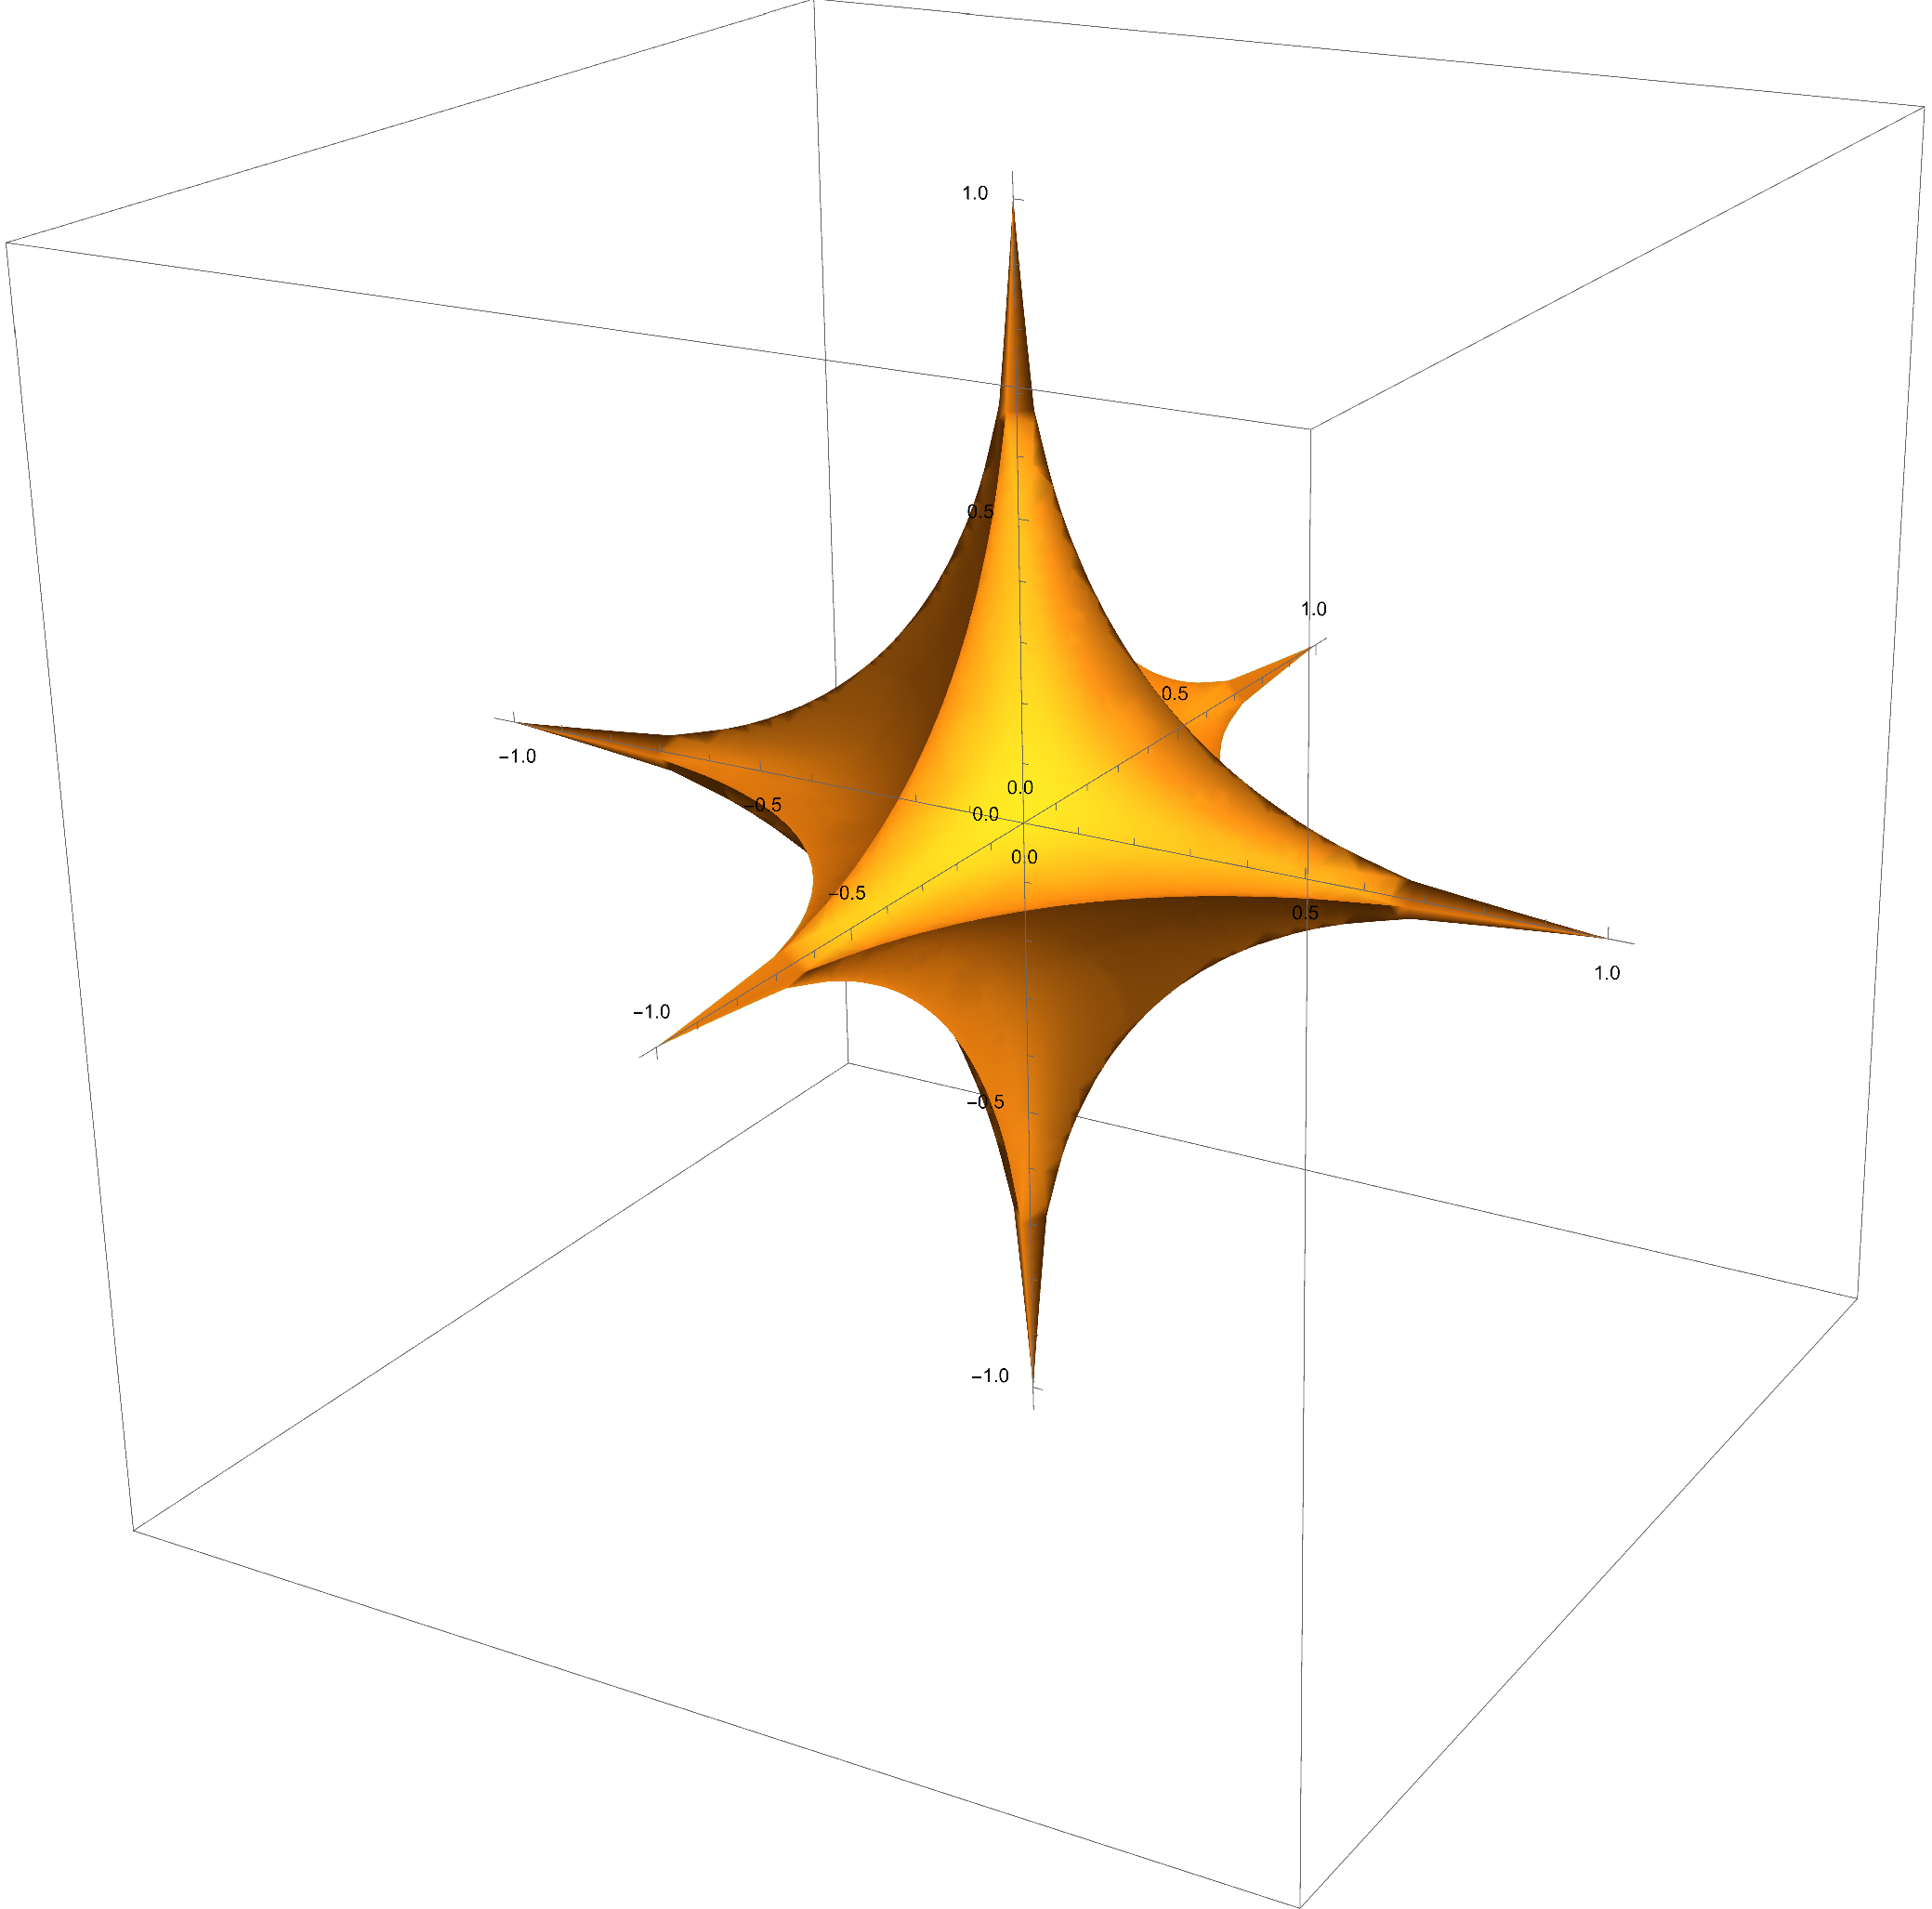
\includegraphics[width=0.5\textwidth]{7. nal slike/zvezdica.pdf}
    \caption[short]{Grafična predstavitev obravnavane oblike ``zvezdice''}
\end{figure}

Poznamo analitičen rezultat za homogeno telo, ko je gostota konstantna ($p=0$): 
\begin{equation}
    m=\frac{4}{45}
\end{equation}
ki ga lahko izračuna \textit{Mathematica}. Rezultat in napako integracije v tem primeru izračunamo:
\begin{equation}
    m \approx \hat{\theta} \pm \sigma = V \,\rho\, \overline{f} \pm \frac{V}{\sqrt{N}}\sqrt{\overline{f^2}-\overline{f}^2}
\end{equation}
kjer je razultat integracije po MMC enak $n/N$ in je $n$ število uspešnih ``zadetkov'' in $N$ vseh poizkusov. Tako dobimo rezulat, ki je odvisen od števila vseh poizkusov, kar je enako iteracijam algoritma, in je prikazan na spodnjih slikah. 

Vidimo, da se pri več iteracijah napaka zmanjšuje z redom $1\sqrt{N}$, kar potrjuje tudi izračunana napaka $\sigma$. Pri $N>10^6$ je rešitev enaka analitični na pribl. 3 decimalna mesta.

Ko smo 1000x pognali simulacijo z enakimi parametri, smo opazovali končni rezultat, ki je bil venomer drugačen, zato smo želeli ugotoviti, ali je mogoče iz več simulacij pri nižjem številu iteracij sklepati o bolj natančni rešitvi kot pri povečevanju števila iteracij. Vidimo, da imamo pri 1000  iteracijah velik raztros rezultatov, ki pa se z povečanjem niža in tako dobimo bolj izrazit vrh pri pričakovani vrednosti $4/45$. Velja pa poudariti, da pri takšnem načinu dosegamo občutno večji računski čas, kot če enostnavno povečamo število iteracij. Ker pa porazdelitev rezultatov spominja na normalno, je lahko srednja vrednost le-te bolj točna in natančna od one, dobljene z povečanimi iteracijami. Te lastnosti bi ne uspeli dobiti, ako bi delali z regularno mrežo, kot je omenjeno v prejšnjem poglavju. Neznano pa nam je, zakaj so rezultati ``kvantizirani'' in ali je to le posledica prikaza.
\begin{figure}[ht]
    \centering
    \begin{minipage}{0.49\textwidth}
        \centering
        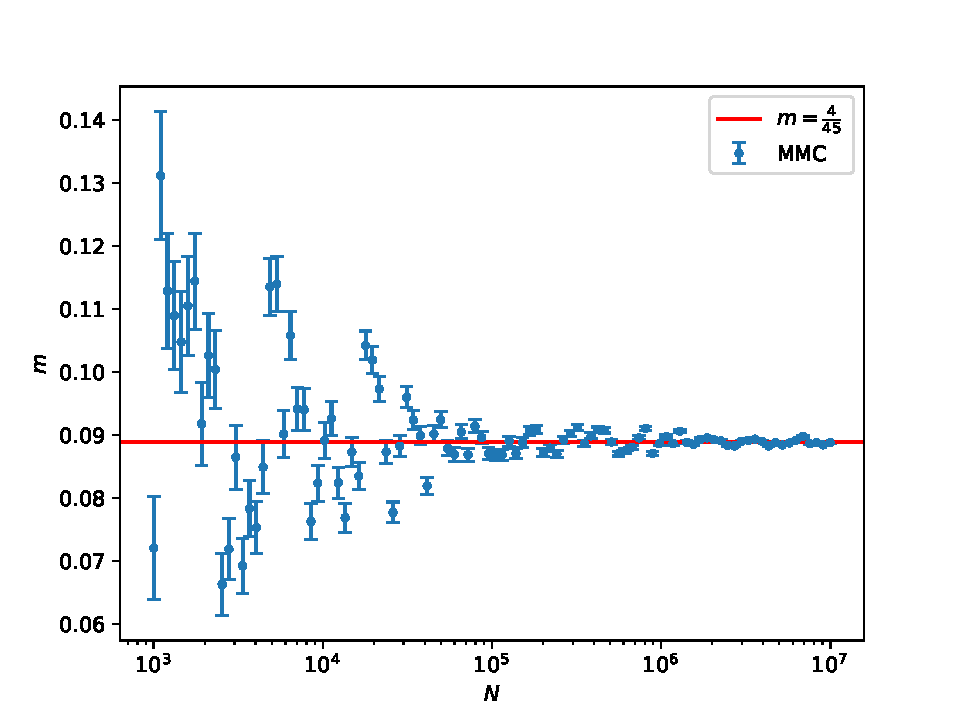
\includegraphics[width=\linewidth]{7. nal slike/masa_N.pdf}
        \caption[short]{Vpliv števila iteracij $N$ na rezultat}
    \end{minipage}
    \begin{minipage}{0.49\textwidth}
        \centering
        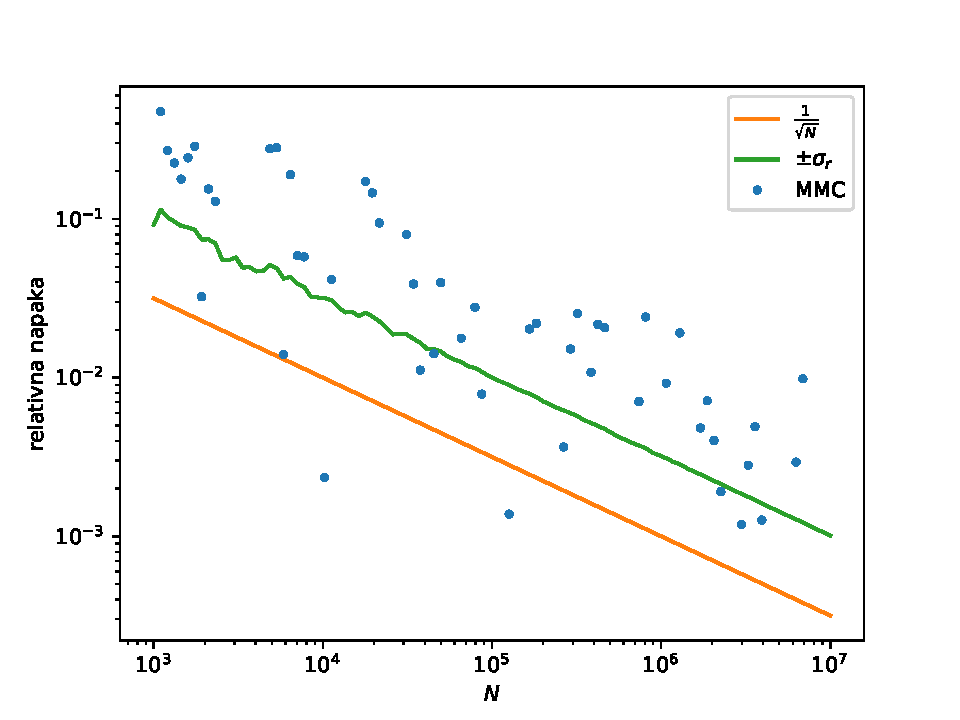
\includegraphics[width=\linewidth]{7. nal slike/masa_relat_napaka.pdf}
        \caption[short]{Vpliv števila iteracij $N$ na relativno napako izračuna}
    \end{minipage}
    \begin{minipage}{0.49\textwidth}
        \centering
        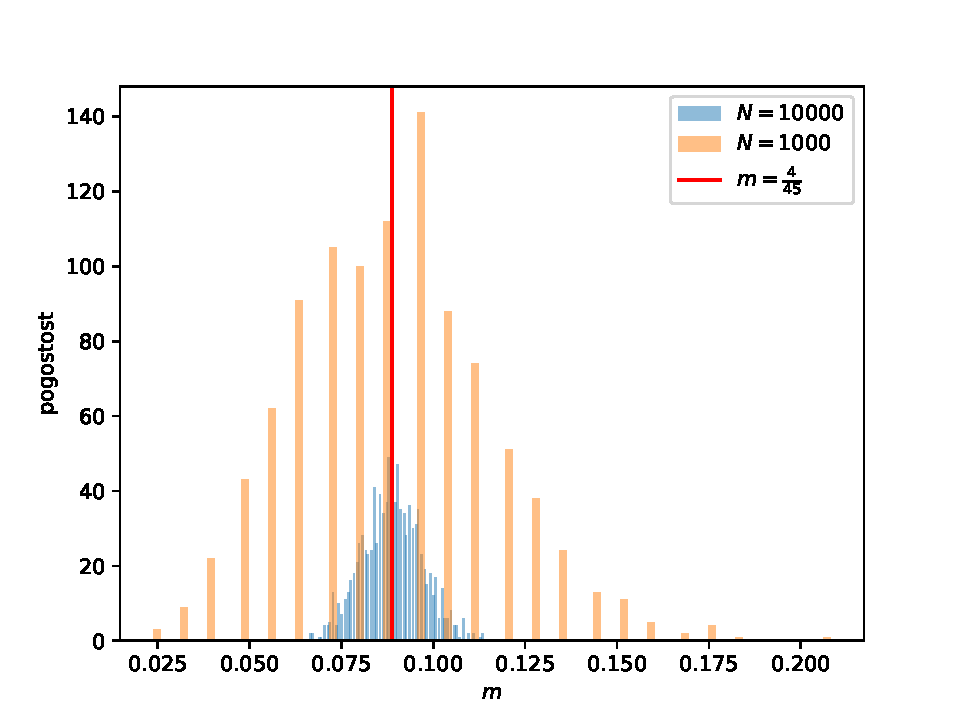
\includegraphics[width=\linewidth]{7. nal slike/masa_porazdelitev.pdf}
        \caption[short]{Histogram pogostosti rezultatov pri ponovitvi istega algoritma 1000x}
    \end{minipage}
\end{figure}

Podobne lastnosti dobimo pri momentih; prvi ali težišče in drugi (masni vztrajnostni -- MVM) moment. Pri tem smo izračunali komponenete lege težišča $\vec{t}$ ter osne in deviacijske masne vztrajnostne momente $J_{ij}$:
\begin{align}
    t_i &= \int_{m}\, x_i \, dm &
    \text{osni MVM: } J_{ii} &= \int_{m}\, (\sum_{j,j\neq i}^{3} x_j^2) \, dm \\
    \text{deviacijski MVM: } J_{ij, j\neq i} &= \int_{m}\, x_i\,x_j \, dm &
    \text{polarni MVM: } J_{p} &= \int_{m}\, (\sum_{i}^{3} x_i^2) \, dm    
\end{align}

Spodnji grafi prikazijejo tudi povprečja in napake izračunov, iz tega lahko sklepamo, da lega težišča in deviacijski MVM težijo k 0, osni in polarni MVM pa k določeni vrednosti. Pri tem je polarni MVM prikazan na posebnem grafu, ker je za red velikosti večji od osnih. Pri tem lahko analitično (to zmore \textit{Mathematica}) izračunamo tudi vrednosti: $J_{ii}= 0,0042328$, nakar nam neskladnost z našimi rezultati ni pojasnjena.
\begin{figure}[ht]
    \centering
    \begin{minipage}{0.49\textwidth}
        \centering
        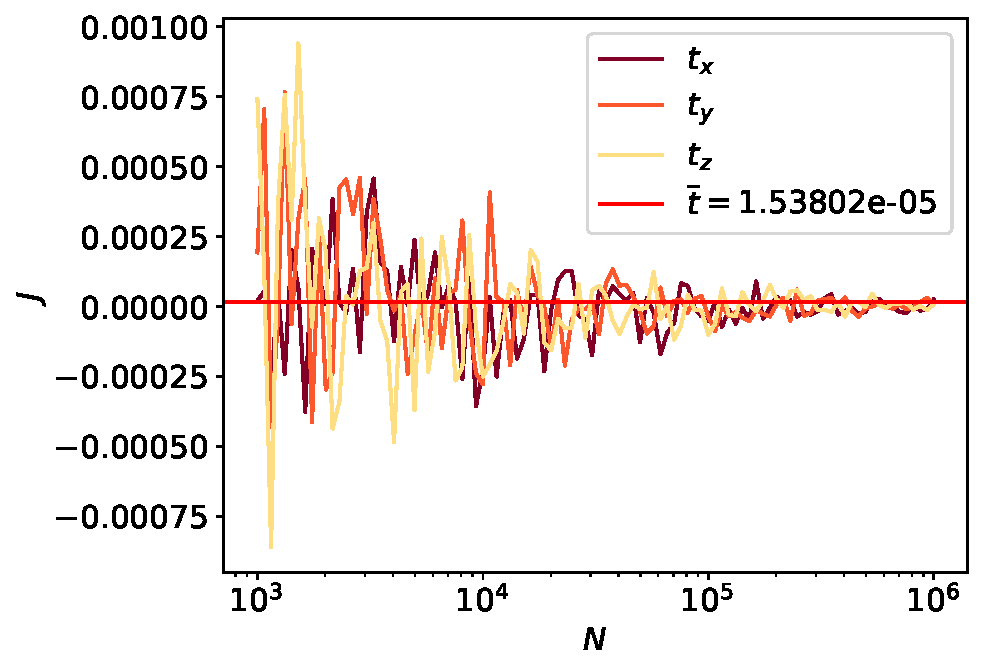
\includegraphics[width=\linewidth]{7. nal slike/težišče.pdf}
        \caption[short]{Odvisnost koordinat lege težišča od $N$}
    \end{minipage}
    \begin{minipage}{0.49\textwidth}
        \centering
        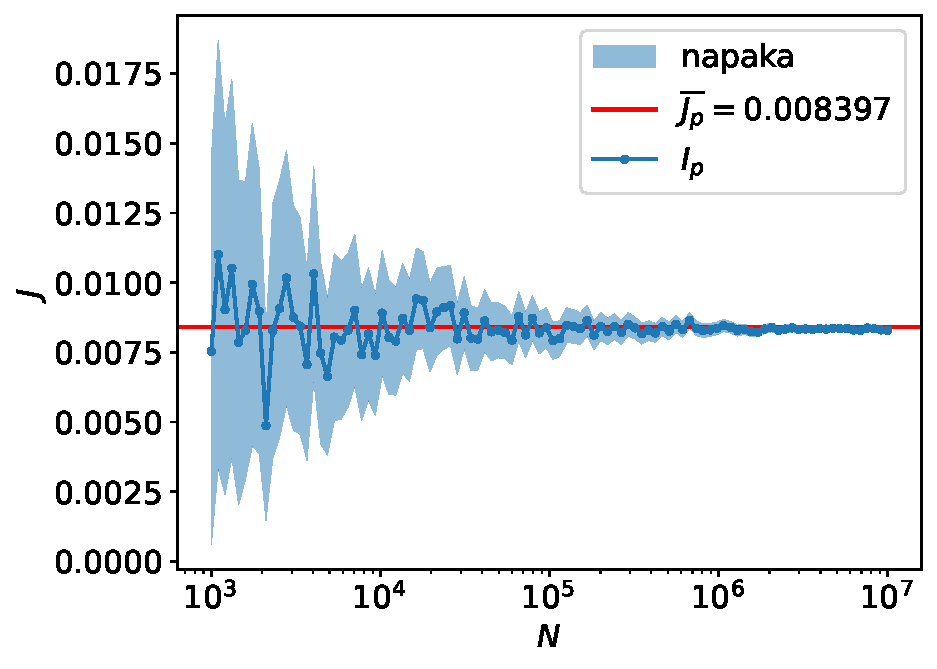
\includegraphics[width=\linewidth]{7. nal slike/J_polarni.pdf}
        \caption[short]{Odvisnost polarnega masnega vztrajnostnega momenta $I_p$ od $N$}
    \end{minipage}
    \begin{minipage}{0.49\textwidth}
        \centering
        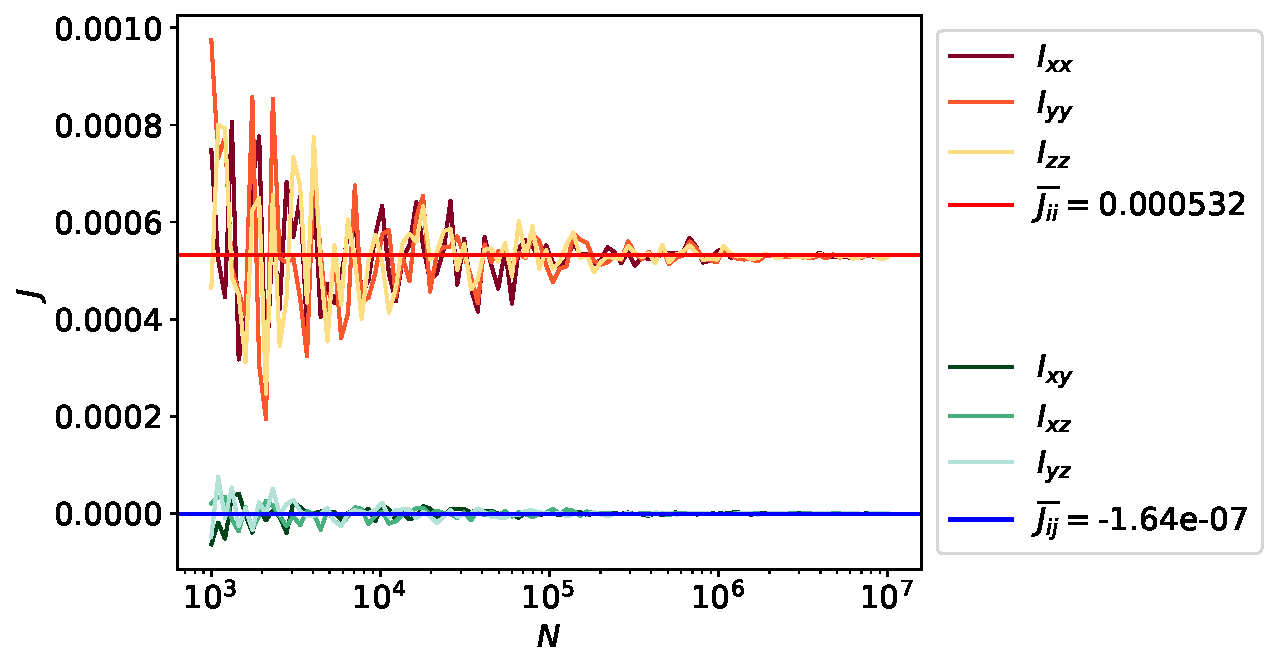
\includegraphics[width=1.25\linewidth]{7. nal slike/mvm.pdf}
        \caption[short]{Odvisnosti masnih vzrtajnostnih momentov od $N$}
    \end{minipage}
\end{figure}

Sedaj primerjamo še odvisnost polarnega MVM, ki je največji od vseh MVM, in mase od parametra $p$ pri nehomogeni gostoti telesa. Opazimo, da nam $p>0$ pomika maso proč od težišča, kjer je sicer manjše telo (kraki zvezdice), vendar to bistveno poveča polarni MVM, saj je več mase bolj proč od težišča. Obratno se dogaja pri $p<0$.
\begin{figure}[ht]
    \centering
    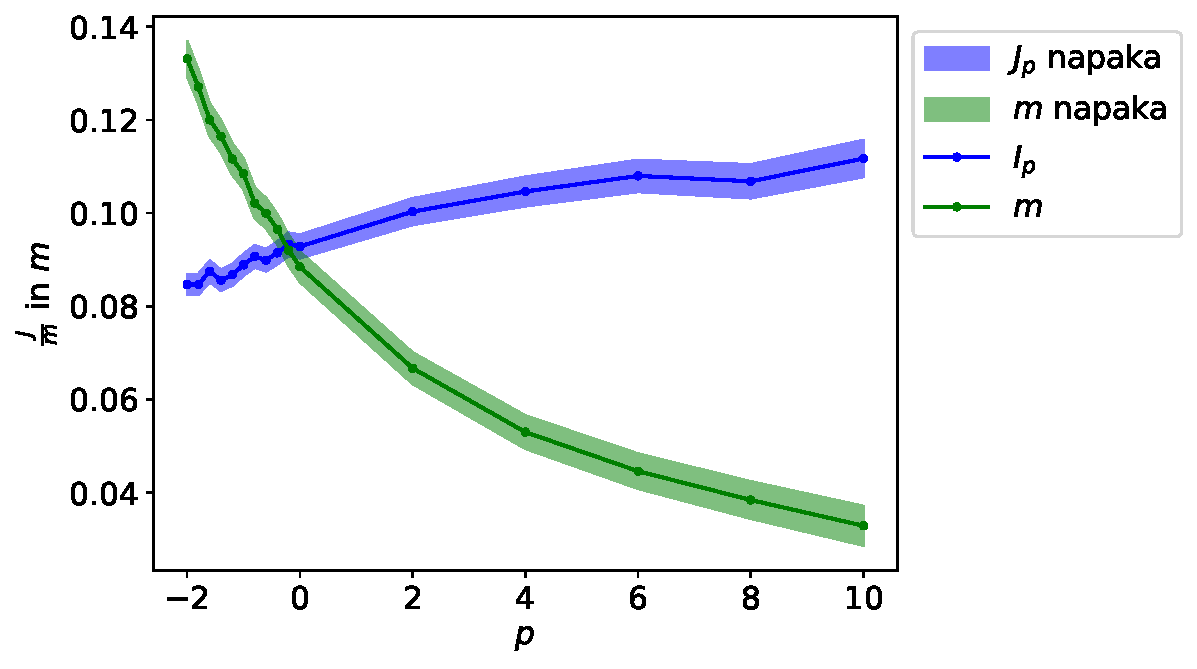
\includegraphics[width=0.6\linewidth]{7. nal slike/Jp_m_vpliv_p.pdf}
    \caption[short]{Vpliv parametra $p$ pri gostoti}
\end{figure}

Če poizkusimo, in se poigramo še z izračunom volumna n-dimenzijske krogle, lahko dobimo sledeča dva grafa za polmer $R=1$ in število izračunov MMC $N=10^6$. Tako opazimo, kako je MMC dober za izračun integralov v več dimenzijah, saj preostale numerične metode tam odpovejo. Ako bi adaptivno povečevali število izračunov, bi lahko tudi pri več dimenzijah dobili rezultate z konstantno napako.

\begin{figure}[ht]
    \centering
    \begin{minipage}{0.49\textwidth}
        \centering
        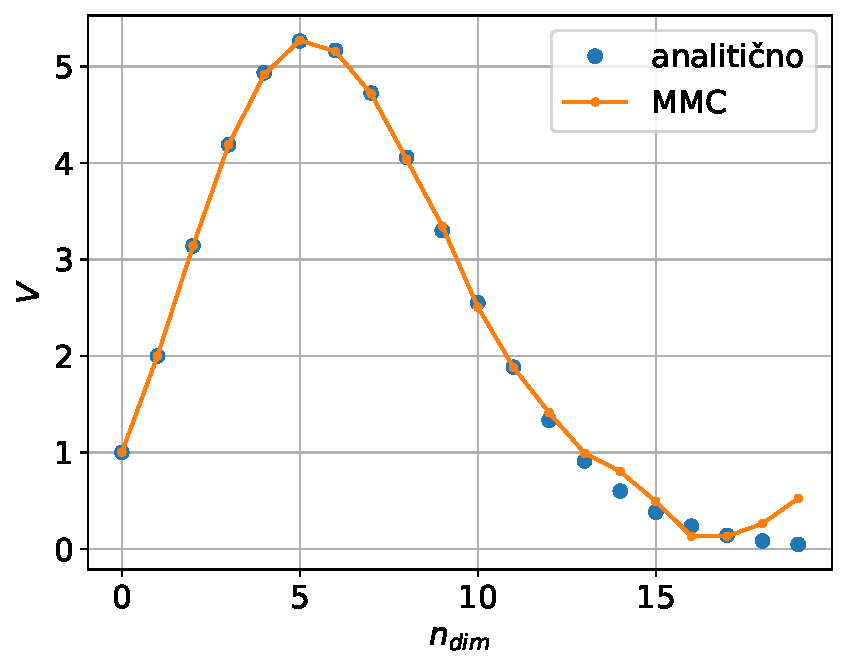
\includegraphics[width=\linewidth]{7. nal slike/vol_ndim.pdf}
        \caption[short]{Volumen n-dimenzijske krogle}
    \end{minipage}
    \begin{minipage}{0.49\textwidth}
        \centering
        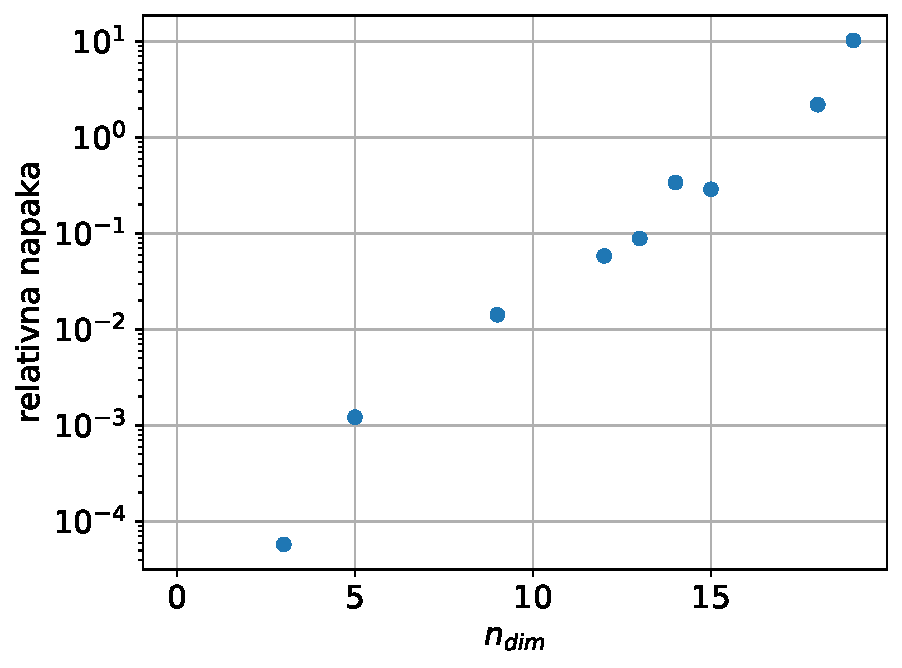
\includegraphics[width=\linewidth]{7. nal slike/vol_ndim_napaka.pdf}
        \caption[short]{Napaka izračuna v primerjavi z analitiko}
    \end{minipage}
\end{figure}

\newpage
\section[]{Žarki gama}

V krogli s polmerom $R$ nastajajo žarki gama s povprečno prosto potjo $\lambda$. Pri tem lahko zapišemo verjetnost, da žarek ``pobegne'' iz krogle, če je dolžina poti žarka $s_i$ porazdeljena eksponentno $f_s(s)=\frac{1}{\lambda}\,e^{-s/\lambda}$:
\begin{equation}
    P=\int_{V} e^{-\frac{d}{\lambda}}\,dV
\end{equation}
kjer je $d$ najmanjša potrebna pot, ki jo mora žarek prepotovati, da pride izven krogle. V našem primeru obravnave v krogu, je to
\begin{equation}
    d(r,\theta) = -r\,\cos\theta + R\,\sqrt{1-\left(\frac{r}{R}\right)^2\,(1-\cos^2\theta)}
\end{equation}
Po metodi Monte Carlo računamo naključno porazdeljene lege po radiju $r_i$ in naključne smeri sevanja $\theta_i$,
\begin{equation}
    r_i = \sqrt[3]{\xi_i}\text{,} \quad \theta_i = \arccos(2\,\xi_i-1)
\end{equation}
kjer je vsako $\xi_i$ nakjučno število na intervalu $[0,1)$. Pri tem preverjamo pogoj pobega $s_i > d(r_i,\theta_i)$ in štejemo ugodne izide. Uvedemo tudi nov parameter: brezdimenzijsko prosto pot $\lambda/R$. Iz rezultatov sledi, da je verjetnost absorbcije žarkov enak $1-P$, kjer je $P$ verjetnost, da žarek pobegne.

\begin{figure}[ht]
    \centering
    \begin{minipage}{0.49\textwidth}
        \centering
        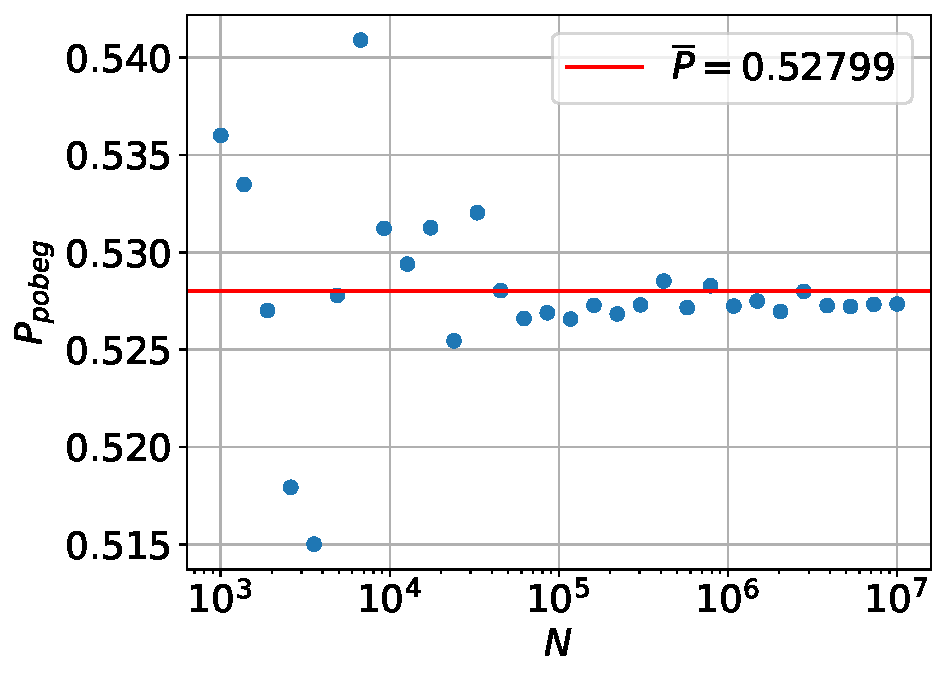
\includegraphics[width=\linewidth]{7. nal slike/gama_N.pdf}
        \caption[short]{Odvisnost rezultata od števila izračunov $N$ pri $\lambda/R=1$}
        \label{fig:gamma_N}
    \end{minipage}
    \begin{minipage}{0.49\textwidth}
        \centering
        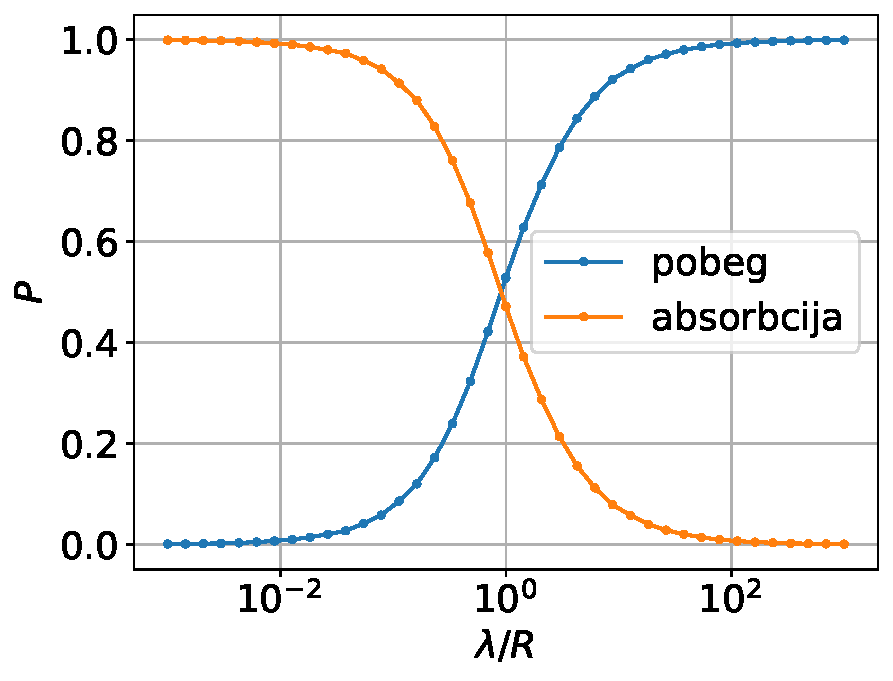
\includegraphics[width=\linewidth]{7. nal slike/gama_pp.pdf}
        \caption[short]{Delež pobeglih in absorbiranih žarkov je odvisen od razmerja $R/\lambda$}
    \end{minipage}
    \begin{minipage}{0.49\textwidth}
        \centering
        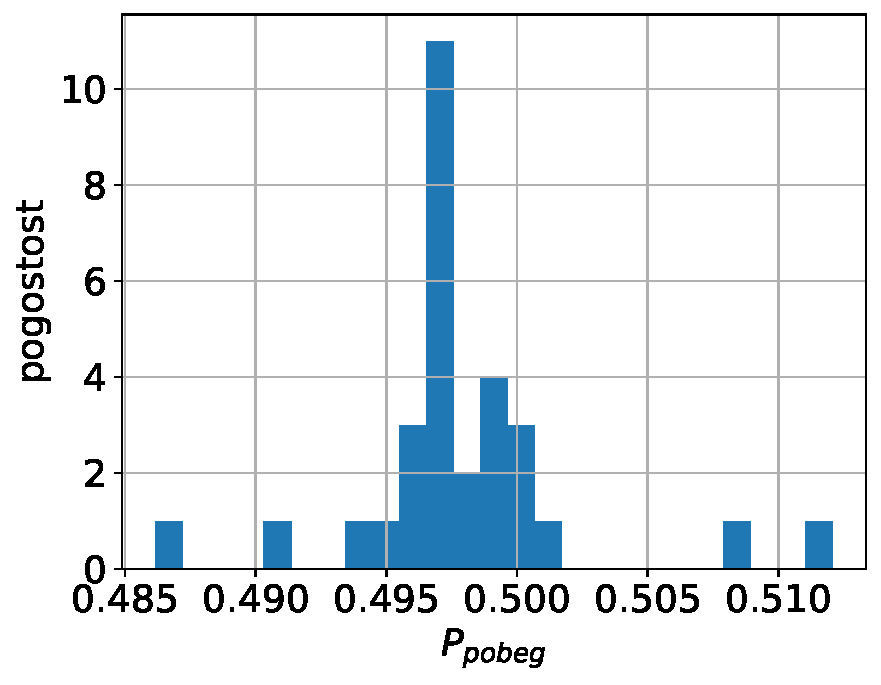
\includegraphics[width=\linewidth]{7. nal slike/gama_porazd.pdf}
        \caption[short]{Porazdelitev rezultatov slike \ref{fig:gamma_N}}
    \end{minipage}
    \begin{minipage}{0.49\textwidth}
        \centering
        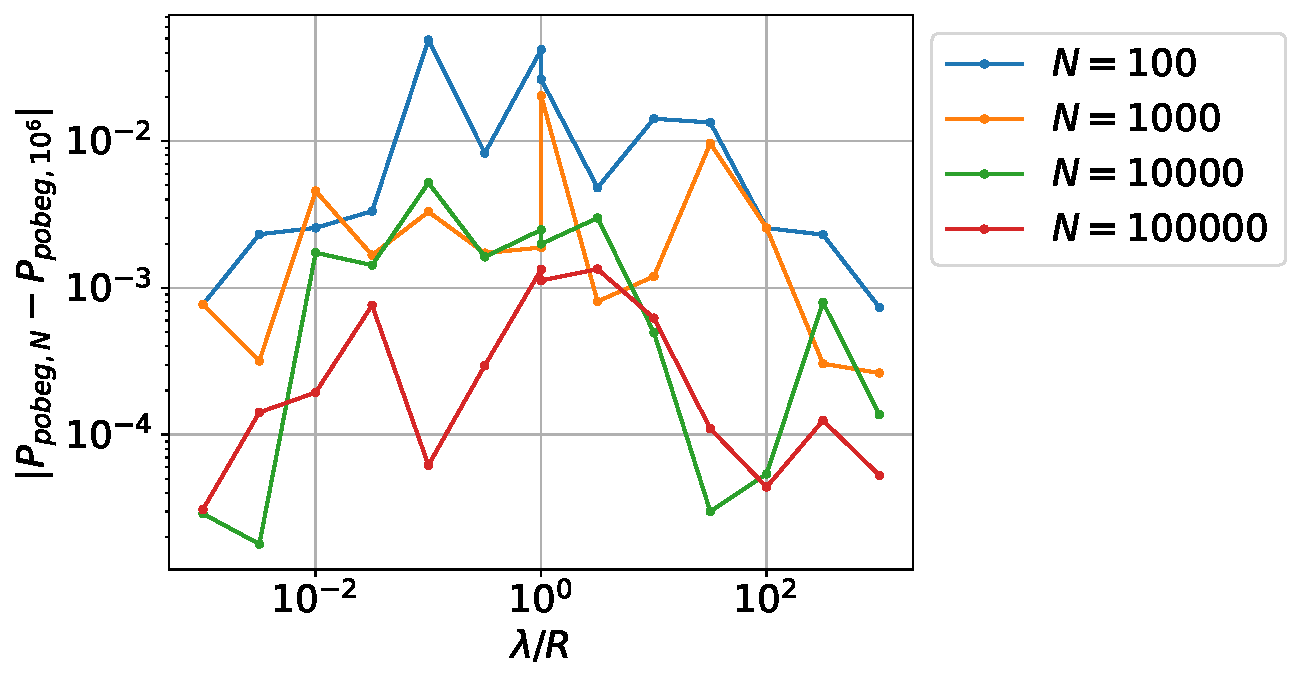
\includegraphics[width=\linewidth]{7. nal slike/gama_napaka.pdf}
        \caption[short]{Napaka v primerjavi s simulacijo z največ iteracijami ($10^6$)}
    \end{minipage}
\end{figure}
Na zgornjih slikah je prikazano, kako se spremijata deleža pobeglih in absorbiranih žarkov v odvisnosti od brezdimenzijske proste poti. Prav tako vidimo, kako se spreminja -- približuje povprečni vrednosti $0,528$ -- verjetnost za pobeg, ako višamo število izračunov. Iz tega lahko sklepamo, da bi bila 0,528 prava vrednost, vedar analitično ali z drugo metodo nismo poizkušali tega potrditi. Pri tem opazimo, da je porazdelitev verjetnosti nesimetrična; pri večjem številu iteracij (nad $10^6$) so vsi rezultati nepričakovano pod povprečjem. Prav tako je prikazana absolutna napaka rezultatov med $10^2$ in $10^6$ izračunov, kjer smo privzeli, da je slednji najbolj točen. Opazimo, da v splošnem napaka pada z večanjem $N$, zanimivo pa je najvišja okoli brezdimenzijske proste poti enake 1.

Sicer pa, ako bi bila $\lambda >> R$ bil delež pobeglih žarkov skoraj 100\% in absorbiranih 0, v limiti, ko $\lambda/R = \inf$, bi tudi bil. Velja tudi obratno, ko $\lambda/R = -\inf$ oziroma je  $\lambda << R$, je delež absorbiranih 100\% in pobeglih 0\%.

Tudi ob spremembi obravne se ta limitna primera ne spreminjata; spremeni se ravnovesno stanje, ko je delež pobeglih enak deležu absorbiranih, kjer smo z zgornjem primeru, 2D krogli predpostavili enake razmere -- porazdelitev -- po polarnem kotu $\phi$.

\vspace{0.5cm}
\newpage
\textbf{Žarki $\mathbf{\gamma}$ v enoosnem elementu}\\
V našem 1D primeru še bolj oklestimo algoritem in izločimo naključno porazdelitev po kotih sevanja $\theta$, kar bi bilo primerno za 1D elemente, kot je npr. dolga in tanka palica krožnega preseka, kjer je sevanje mogoče le v eni -- osni smeri. Recimo, da je palica nekako izolirana, kar preprečuje izhod v radialni smeri. Tako žrebamo le lego $l_i$ enakomerno po intervalu [0,1) in dolžino poti delčka $s_i$ po eksponentni porazdelitvi kot poprej. Tokrat preverjamo pogoj pobega bolj preprosto:
\begin{equation}
    s_i > d(l_i) = L - l_i
\end{equation}
kjer je $L$ dolžina palice. Tukaj opazimo večji delež pobeglih žarkov in hitrejšo konvergenco.

\vspace{0.5cm}
\textbf{Žarki $\mathbf{\gamma}$ v krogli v treh dimenzijah}\\
Ako pa problem obranavamo v treh dimenzijah, torej pravi krogli, pa upoštevamo porazdelitev lege po polmeru $r_i= \sqrt[3]{\xi_i}$ in po azimutu $\theta_i= \arccos(2\,\xi_i-1)$ enako kot v 2D, kjer dodamo porazdelitev po polarnem $\phi_i = 2\,\pi\,\xi_i$. Prav tako žrebamo porazdelitev smeri izsevanega žarka v azimutni smeri enako kot v 2D $\theta_{\text{sev,}i}= \arccos(2\,\xi_i-1)$ in dodamo polarno smer $\phi_{\text{sev,}i} = 2\,\pi\,\xi_i$. Prosta pot $s_i$ se žreba eksponentno, vse ostalo pa enakomerno po intervalu [0,1). Tokrat je izraz za $d$ bolj kompleksen:
\begin{equation}
    s > d(r_i,\phi_i,\theta_i,\phi_{\text{sev,}i},\theta_{\text{sev,}i}) = R - r\,\cos\alpha
\end{equation}
kjer je $\alpha$ kot med smerjo sevanja $(\phi_{\text{sev,}i},\theta_{\text{sev,}i})$ in krajevnim vektorjem točke izsevanja $(r_i,\phi_i,\theta_i)$ in znaša:
\begin{equation}
    \cos\alpha = \cos\phi_i\,\sin\theta_i\,\cos\phi_{\text{sev,}i}\,\sin\theta_{\text{sev,}i} + \sin\phi_i\,\sin\theta_i\,\sin\phi_{\text{sev,}i}\,\sin\theta_{\text{sev,}i} + \cos\theta\,\cos\theta_{\text{sev,}i}
\end{equation}

\begin{figure}[ht]
    \centering
    \begin{minipage}{0.49\textwidth}
        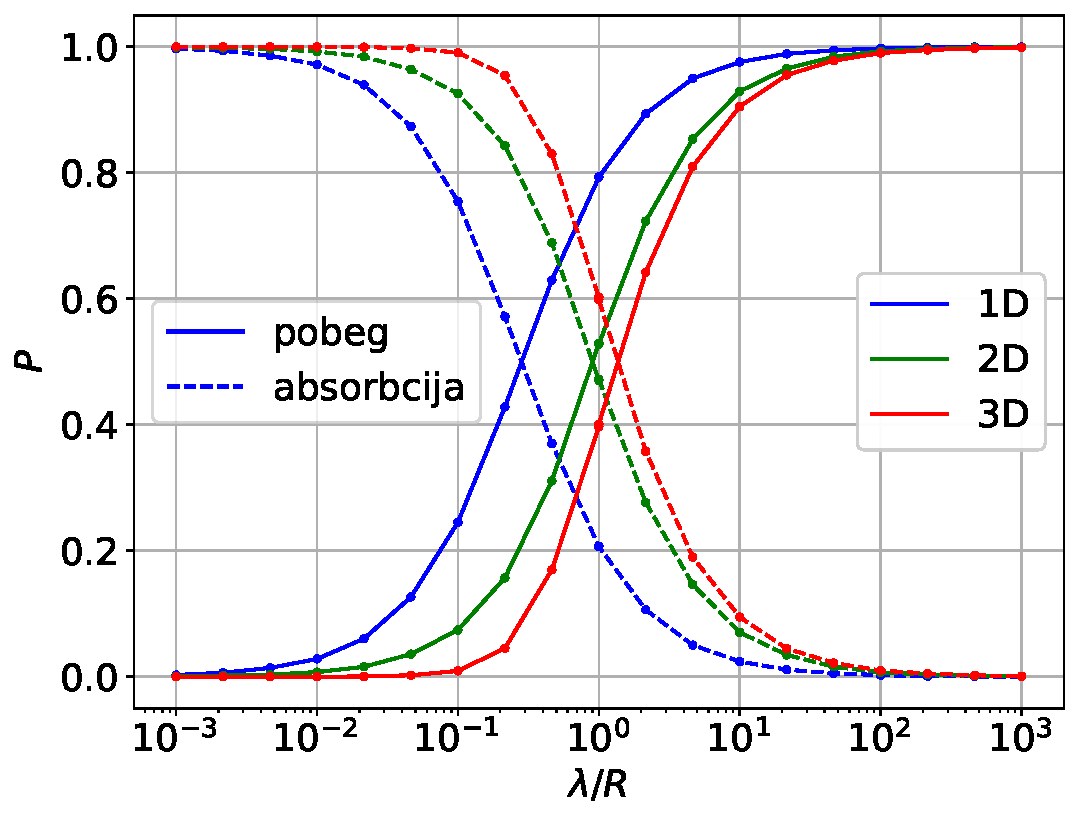
\includegraphics[width=\linewidth]{7. nal slike/gama_pp_1D_2D_3D.pdf}
        \caption[short]{Primerjava algoritmov}
    \end{minipage}
    \begin{minipage}{0.49\textwidth}
        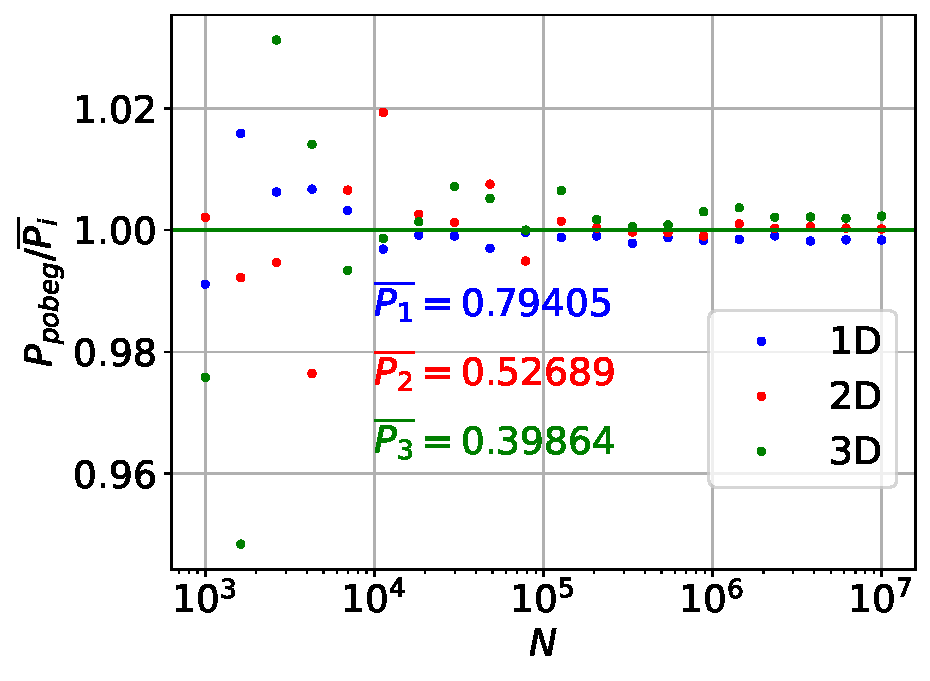
\includegraphics[width=\linewidth]{7. nal slike/gama_N_vse_dim.pdf}
        \caption[short]{Izračuni za $\lambda/R=1$}
    \end{minipage}
\end{figure}
Opazimo, da predvsem v bližini $\lambda/R=1$ dobimo različne rezultate, pri obravnavi v različnih dimezijah. Razlika izgleda največja ravno pri $\lambda/R=1$, zato je za ta izsek prikazano bolj natančno na dasno sliki. Na limitne primere to nima vpliva.

V tem primeri velja tudi poudariti, da takšne obravnave terjajo različne računske čase; osnovni 2D primer ima pribl. 3x večji računski čas od 1D in za polovico manjšega od 3D primera. Na to vpliva predvsem generacija naključnih števil, za katero smo uporabljali funkciji \texttt{random} in \texttt{exponential} iz knjižnice \texttt{numpy.random}. Mogoče bi se katera druga implementacija psevdo-naključnih števil lahko izkazala za učinkovitejšo.

\section[]{Nevtronski reflektor}

Predpostavimo preprost 1D reflektor, kjer je mogoče premikanje in sipanje delcev le v eni osi. Pri tem v duhu Monte Carla žrebamo naključno smer sipanja $b$ binarno ($b=1$ naprej in $b=-1$ nazaj) ter prosto pot $s_i$ po eksponentni porazdelitvi, tako kot v prejšnjem poglavju.

V naslednjem koraku preverimo, kje se nahaja delec glede na dolžino medija $L$, če je izhodišče $x=0$ na začetku medija:
\begin{itemize}
    \item če $x_i > L$: nevtron je prepuščen in 
    \item če $x_i<0$: nevtron je odbit,
\end{itemize}
kjer je $x_i$ lega delca, izračunana iterativno za vsak naslednji korak 
\begin{equation}
    x_{i,j+1}= x_{i,j} + b\,s_i
\end{equation}

Začetne pogoje smo definirali na tak način, da vsi nevtroni vpadejo v madij pri $x=0$ in se lahko tam sipljejo le naprej $b=1$ po eksponentno porazdeljeni prosti poti. V sledečem algoritmu smo beležili števila prepuščenih in odbitih nevtronov ter število sipanj vsakega delčka. Na grafih $N$ predstavlja število dalcev na začetku, kjer smo vsak nevtron sipali, dokler ni zapustil medija in $\lambda/L$ brezdimenzijsko povprečno prosto pot, podobno kot v prejšnjem poglavju.

\begin{figure}[ht]
    \centering
    \begin{minipage}{0.49\textwidth}
        \centering
        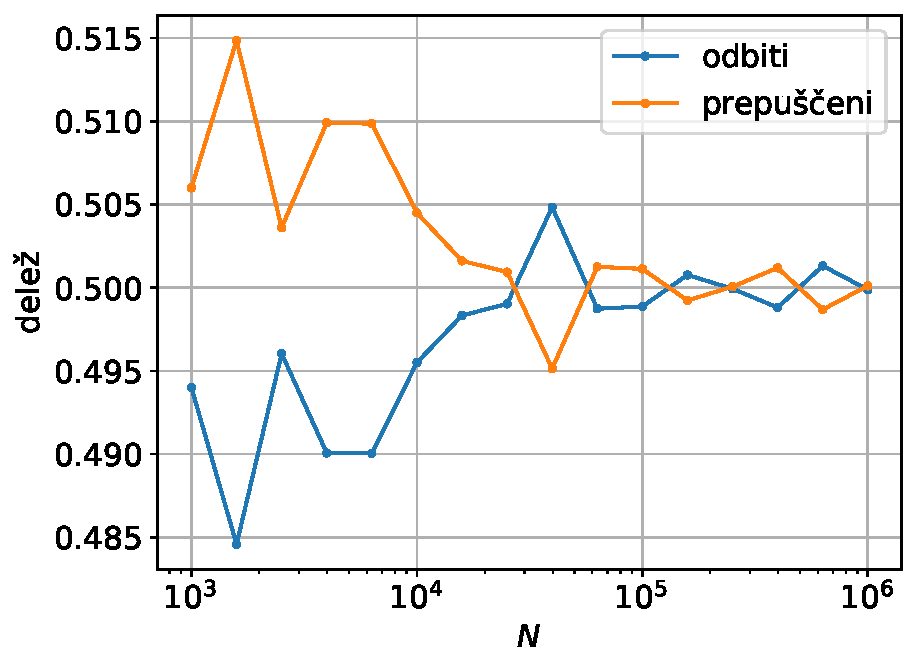
\includegraphics[width=\textwidth]{7. nal slike/nevtroni_N.pdf}
        \caption[short]{Konvergenca izračuna glede na število delcev $N$}
    \end{minipage}
    \begin{minipage}{0.49\textwidth}
        \centering
        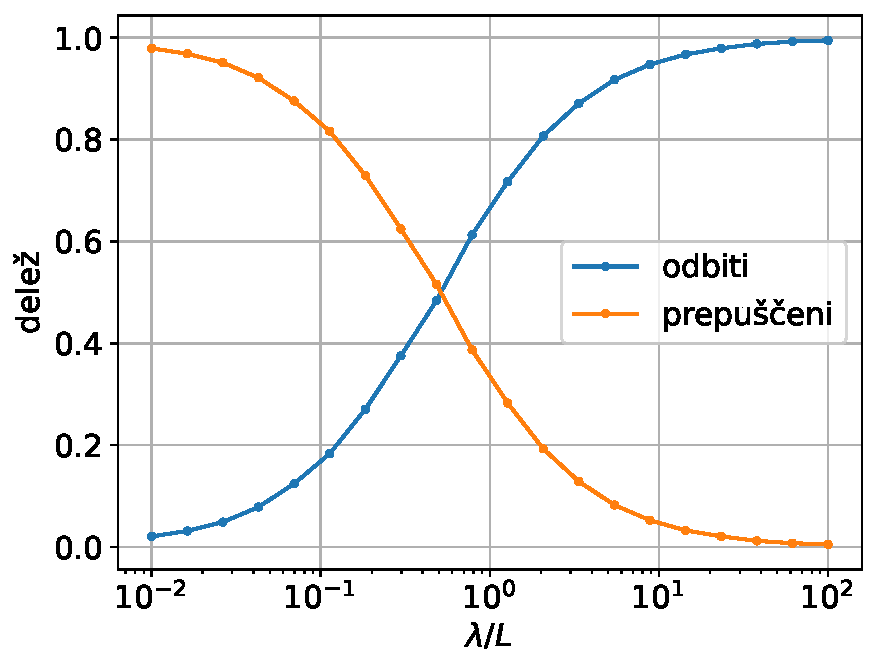
\includegraphics[width=\textwidth]{7. nal slike/nevtroni_pp.pdf}
        \caption[short]{Odvisnost prepustnosti in odbojnosti od brezdimenzijske povprečne proste poti}
    \end{minipage}
\end{figure}

Vsi rezultati, razen na prvi sliki, so izračunani za $N=20 000$ delcev, kar omogoča natančno a še vedno hitro računanje. Opazimo, da ima graf podobno obliko, kot v prejšnji nalogi; pri $\lambda >> L$ prevladuje odbojnost in ko $\lambda <<L$ prepustnost.

Porazdelitev na spodnji sliki več kot očitno pri $\lambda >>L$ teži k nič, in k nekakakšni eksponentni porazdelivi pri $\lambda <<L$, kar je smiselno, ker v prvem primeru skoraj ne prihaja do sipanj, saj večina pride skozi medij že v prvem koraku, prosta pot pa je porazdeljena eksponentno.

\begin{figure}[ht]
    \centering
    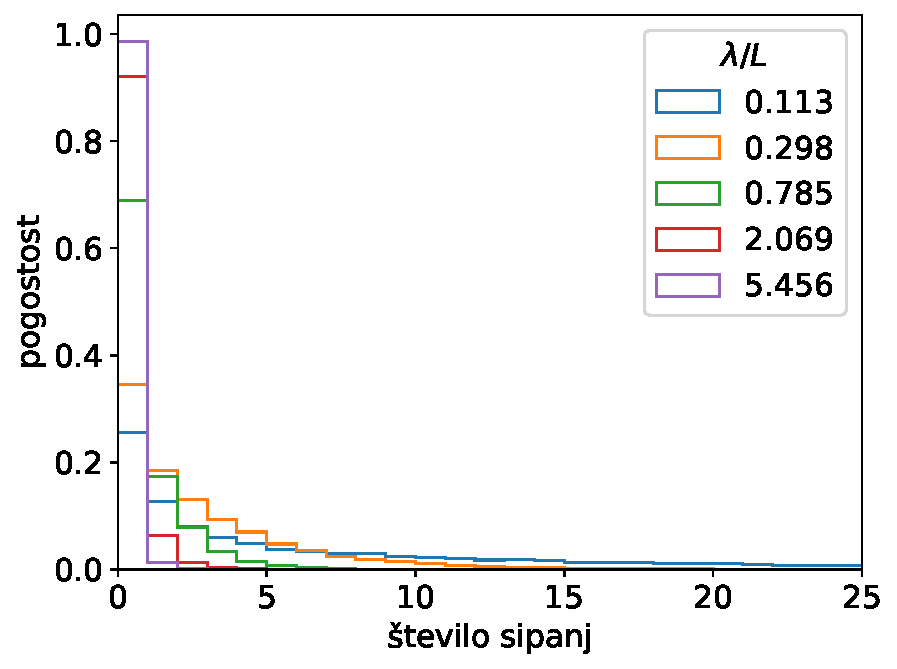
\includegraphics[width=0.5\textwidth]{7. nal slike/nevtroni_porazd_pp.pdf}
    \caption[short]{Normirana porazdelitev števila sipanj v 1D glede na brezdimenzijsko povprečno prosto pot}
\end{figure}

Zaženemo še 2D primer, ko sipanje ni več le v eni dimenziji, ampak predpostavimo enakomerno sipanje pod kotom $\alpha$ žrebanem naključno med $\alpha_i=2\,\pi\,\xi_i$. Pri tem moramo spremeniti tudi izračun lege delca. Ker nas zanima le lega v x-smeri, saj nam ta pove, ali je delec zapustil medij, le-to izračunamo sledeče
\begin{equation}
    x_{i,j+1}= x_{i,j} + \cos(\alpha_i)\,s_i
\end{equation}

\begin{figure}[ht]
    \centering
    \begin{minipage}{0.4\textwidth}
        \centering
        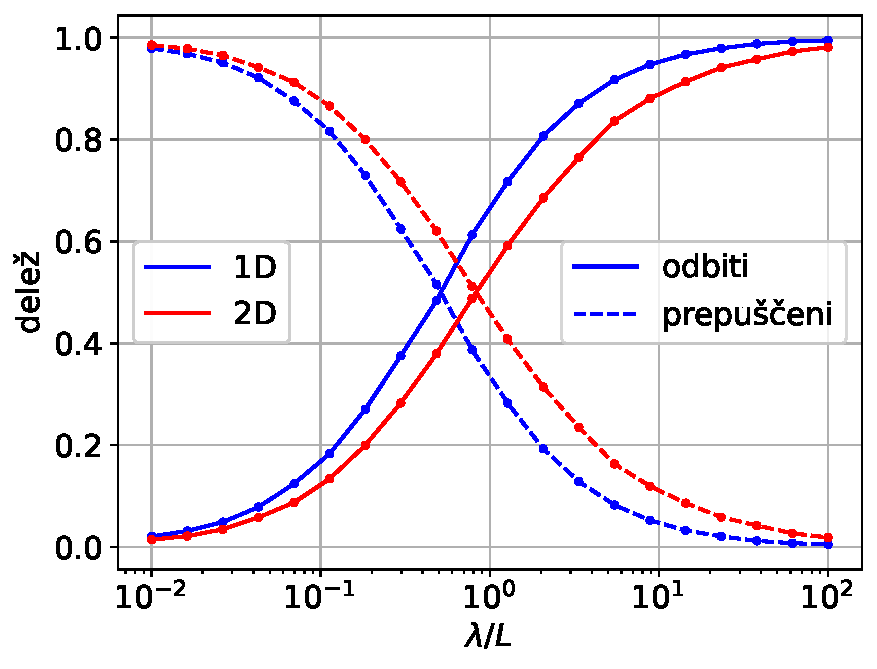
\includegraphics[width=\textwidth]{7. nal slike/nevtroni_pp_2D.pdf}
        \caption[short]{Prepustnost in odbojnost primerjava med 1D in 2D}
    \end{minipage}
    \begin{minipage}{0.4\textwidth}
        \centering
        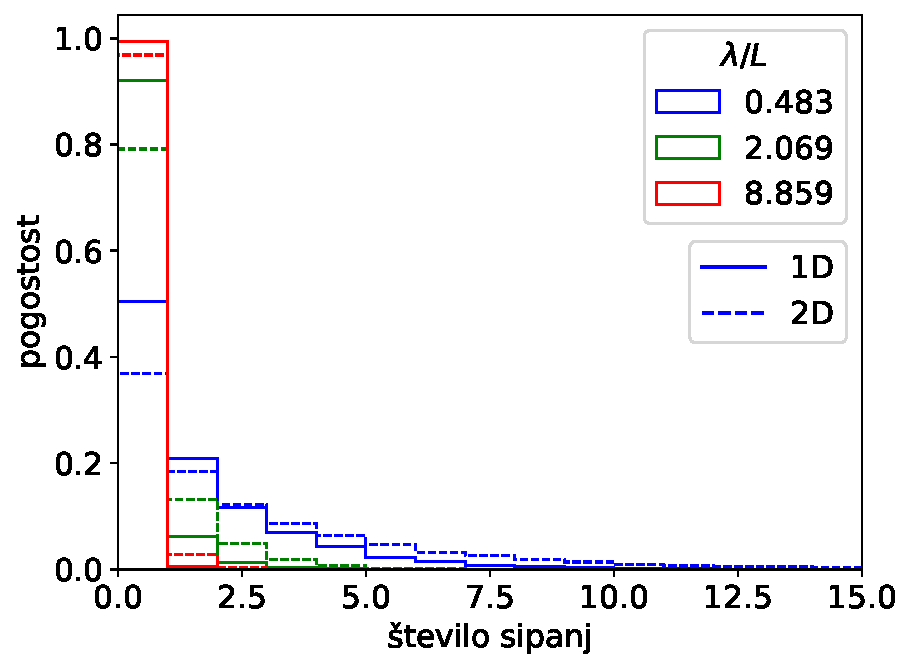
\includegraphics[width=\textwidth]{7. nal slike/nevtroni_porazd_2_1D.pdf}
        \caption[short]{Normirana porazdelitev števila sipanj v primerjavi med 2D in 1D}
    \end{minipage}
\end{figure}

Ako pa si domislimo še 3D primer, kjer dodamo porazdelitev sipanja še po kotu v z-osi $\beta_i=2\,\pi\,\xi_i$, se izraz za lego nevtrona spremeni, ostalo pa ostane identično.
\begin{equation}
    x_{i,j+1}= x_{i,j} + \cos(\alpha_i)\,\cos(\beta_i)\,s_i
\end{equation}

Na spodnji sliki opazimo, da vsaka dodana dimenzija premika graf v desno. Pri tem se prepustnost manjša, kar je pričakovano, glede na dodane nove smeri sipanj. Tako je v 1D ravnovesna lega (ko je prepustnost enaka odbojnosti) pri $\lambda/L=0,5$, v 2D pri pribl. 0,85 in v 3D pri 1,5.

\begin{figure}[ht]
    \centering
    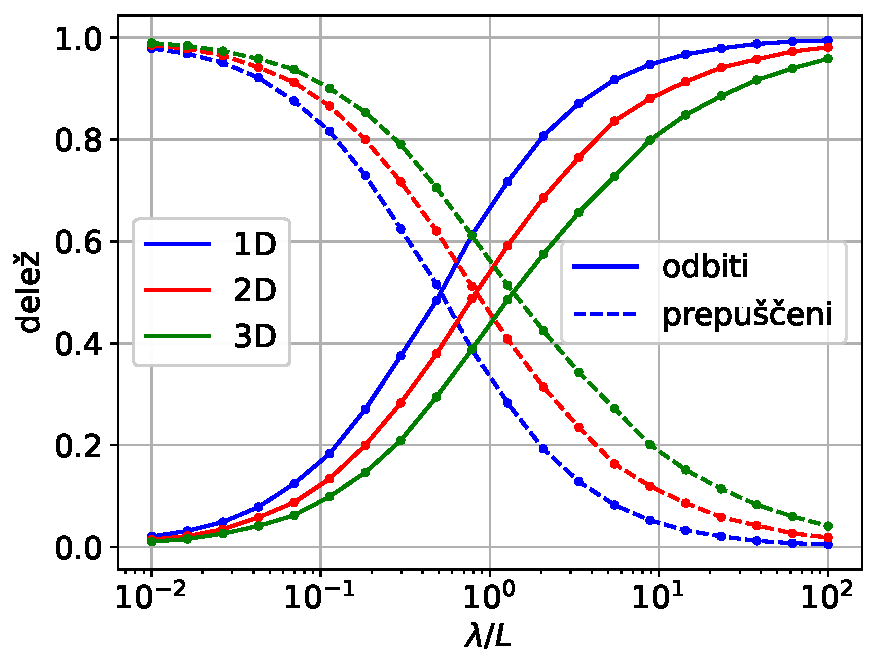
\includegraphics[width=0.45\linewidth]{7. nal slike/nevtroni_pp_3D.pdf}
    \caption[short]{Primerjava vseh dimenzij}
\end{figure}

Lahko se še malo igramo z porazdelitvami sipanja pod kotom v 3D, kjer smo poizkušali doseči anizotropno sipanje. Zanimivo je, da uporaba normalne porazdelitve praktično nima vpliva na prepustnost, dočim Weibullova pri oblikovnem parametru $k>1$ vpliva na spremembo oblike krivulje prepustnosti. O fizikalni pravilnosti takega sipanja sicer nisem prepričan.
\begin{figure}[ht]
    \centering
    \begin{minipage}{0.45\textwidth}
        \centering
        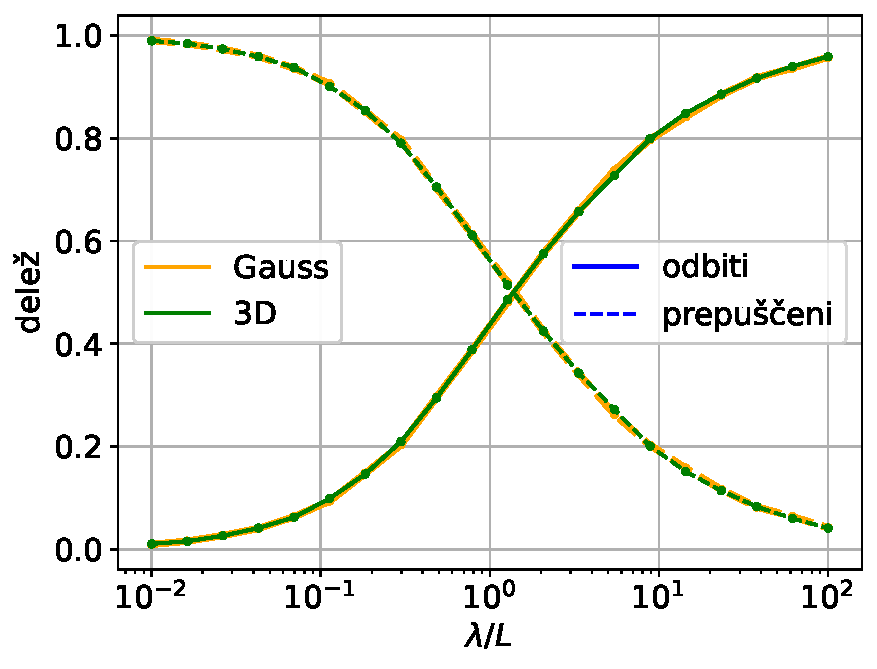
\includegraphics[width=\linewidth]{7. nal slike/nevtroni_pp_gauss.pdf}
        \caption[short]{Gauss-ova porazdelitev}
    \end{minipage}
    \begin{minipage}{0.45\textwidth}
        \centering
        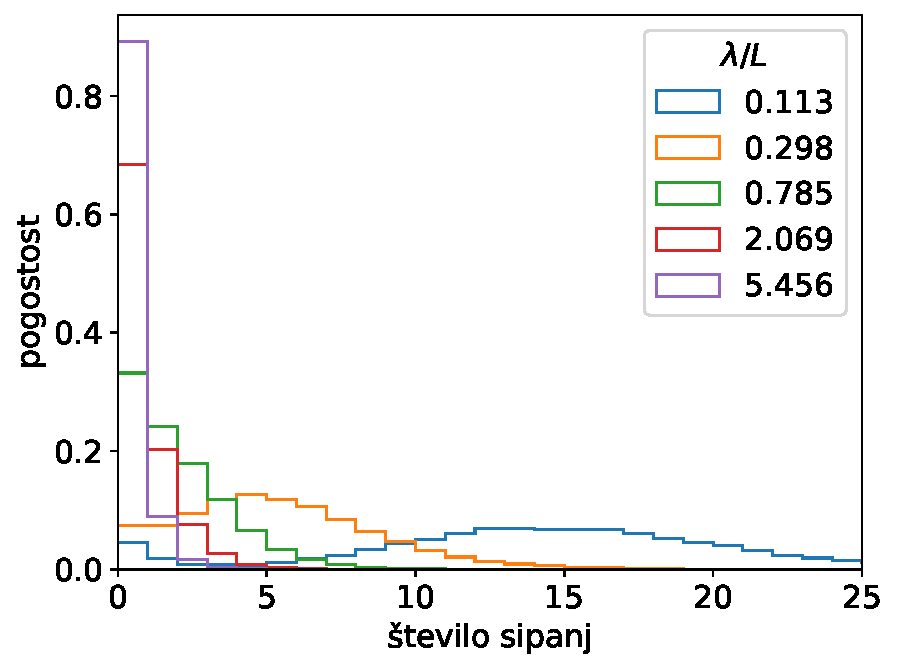
\includegraphics[width=\linewidth]{7. nal slike/nevtroni_porazd_pp_w10.pdf}
        \caption[short]{Porazdelitev števila sipanj pri Weibullovi porazdelitvi kotov z $k=10$}
    \end{minipage}
    \begin{minipage}{0.45\textwidth}
        \centering
        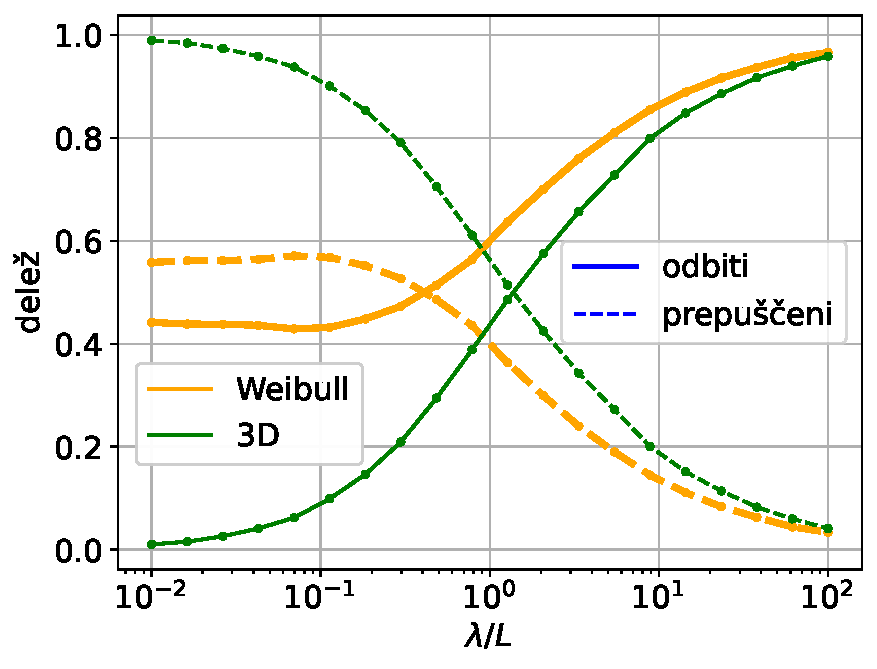
\includegraphics[width=\linewidth]{7. nal slike/nevtroni_pp_w5.pdf}
        \caption[short]{Weibull-ova porazdelitev $k=5$}
    \end{minipage}
    \begin{minipage}{0.45\textwidth}
        \centering
        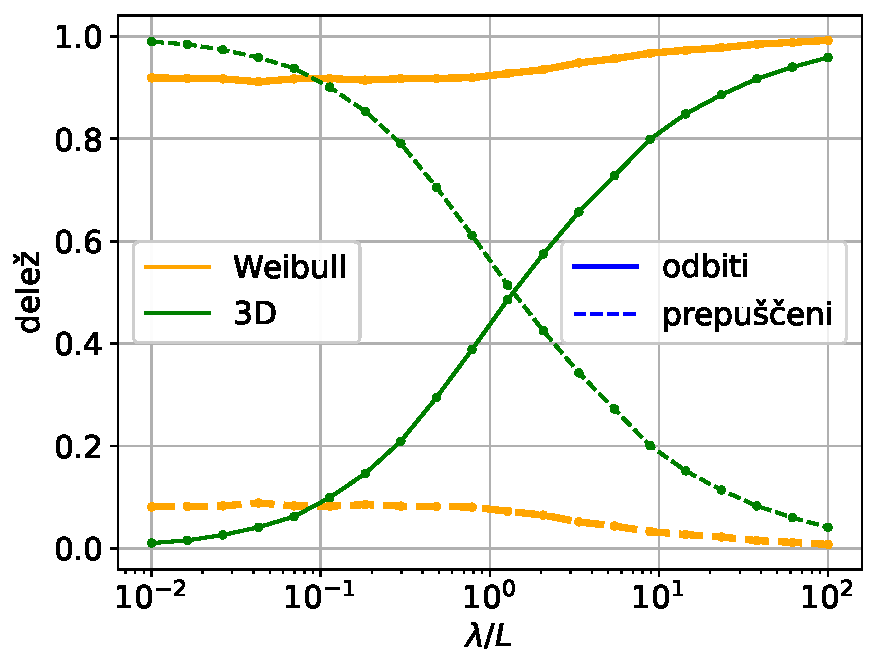
\includegraphics[width=\linewidth]{7. nal slike/nevtroni_pp_w10.pdf}
        \caption[short]{Weibull-ova porazdelitev $k=10$}
    \end{minipage}
\end{figure}